
\dev{Marin Malory}{\cite{Motwani}}

\textit{Ce développement a pour but d'étudier la complexité moyenne du tri rapide randomisé, et s'intègre ainsi naturellement dans la leçon \ref{L8}. 
Puisque cet algorithme est probabiliste et utilise le paradigme \og diviser pour régner \fg{} , il peut aussi servir d'illustration dans les leçons \ref{L11} et\ref{L12}. }\newline


Le but est de montrer le théorème suivant, qui analyse le temps d'exécution moyen du tri rapide randomisé (pour le pseudo-code, voir \ref{TriRandom}).

\begin{theorem}
L'espérance du nombre de comparaisons du tri rapide randomisé d'un ensemble à $n$ éléments est au plus $2nH_n$ où $H_n$ est le terme général de la série harmonique.
\end{theorem}

\begin{proof}
Soit $T$ un tableau à $n$ éléments. Pour $1\leq i \leq n$, on note $t_i$ le $i$-ème plus petit élément de $T$. Ainsi, $t_1 = \min T$ et $t_n = \max T$. On pose $X_{ij}$ la variable aléatoire valant $1$ si $t_i$ et $t_j$ sont comparés au cours de l'exécution, et $0$ sinon. 

On remarque alors que deux éléments $t_i$ et $t_j$ sont comparés au plus une fois. En effet, si $t_i$ et $t_j$ sont comparés , l'un des deux était un pivot et n'est comparé avec plus personne ensuite.

Ainsi, le nombre total de comparaisons est $N = \sum_{1\leq i <j \leq n} X_{ij}$. Par linéarité de l'espérance, on a alors 
$$
\mathbb{E}(N) = \sum_{1\leq i<j \leq n} \mathbb{E}(X_{ij})
$$
En notant $p_{ij} = \mathbb{P}(X_{ij}=1)$, on a directement $\mathbb{E}(X_{ij}) =p_{ij}$.

\begin{lemma}
Pour tout $1\leq i <j \leq n$, on a $p_{ij} = \frac{2}{j-i+1}$.
\end{lemma}

On peut voir l'exécution du tri rapide comme un arbre binaire, avec comme nœuds les pivots successifs. On note alors $\pi$ la permutation de $T$ obtenu en faisant un parcours en largeur de l'arbre obtenu. L'arbre ci-dessous représente l'exécution du tri rapide sur un tableau à $9$ éléments. On a ici $\pi = (4,8,2,5,1,9,6,3,7)$.
\begin{center}
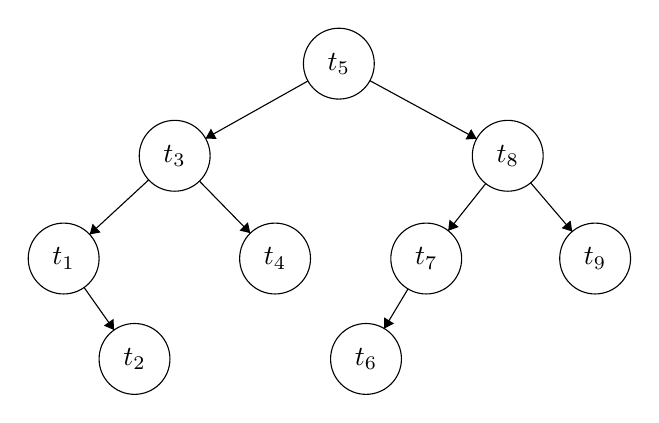
\begin{tikzpicture}[scale=0.15]
\tikzstyle{every node}+=[inner sep=0pt]
\draw [black] (36.6,-13.3) circle (3);
\draw (36.6,-13.3) node {$t_5$};
\draw [black] (22.7,-21.1) circle (3);
\draw (22.7,-21.1) node {$t_3$};
\draw [black] (50.9,-21.1) circle (3);
\draw (50.9,-21.1) node {$t_8$};
\draw [black] (31.2,-29.8) circle (3);
\draw (31.2,-29.8) node {$t_4$};
\draw [black] (13.3,-29.8) circle (3);
\draw (13.3,-29.8) node {$t_1$};
\draw [black] (19.3,-38.3) circle (3);
\draw (19.3,-38.3) node {$t_2$};
\draw [black] (44,-29.8) circle (3);
\draw (44,-29.8) node {$t_7$};
\draw [black] (58.3,-29.8) circle (3);
\draw (58.3,-29.8) node {$t_9$};
\draw [black] (38.9,-38.3) circle (3);
\draw (38.9,-38.3) node {$t_6$};
\draw [black] (33.98,-14.77) -- (25.32,-19.63);
\fill [black] (25.32,-19.63) -- (26.26,-19.68) -- (25.77,-18.8);
\draw [black] (39.23,-14.74) -- (48.27,-19.66);
\fill [black] (48.27,-19.66) -- (47.8,-18.84) -- (47.32,-19.72);
\draw [black] (20.5,-23.14) -- (15.5,-27.76);
\fill [black] (15.5,-27.76) -- (16.43,-27.59) -- (15.75,-26.85);
\draw [black] (24.8,-23.25) -- (29.1,-27.65);
\fill [black] (29.1,-27.65) -- (28.9,-26.73) -- (28.19,-27.43);
\draw [black] (49.04,-23.45) -- (45.86,-27.45);
\fill [black] (45.86,-27.45) -- (46.75,-27.13) -- (45.97,-26.51);
\draw [black] (52.84,-23.39) -- (56.36,-27.51);
\fill [black] (56.36,-27.51) -- (56.22,-26.58) -- (55.46,-27.23);
\draw [black] (15.03,-32.25) -- (17.57,-35.85);
\fill [black] (17.57,-35.85) -- (17.52,-34.91) -- (16.7,-35.48);
\draw [black] (42.46,-32.37) -- (40.44,-35.73);
\fill [black] (40.44,-35.73) -- (41.28,-35.3) -- (40.43,-34.78);
\end{tikzpicture}
\end{center}

\begin{proof}
On peut faire deux remarques :
\begin{enumerate}
\item $t_i$ et $t_j$ sont comparés ssi pour tout $i<l<j$, $\pi(t_i) \leq \pi(t_l)$ et $\pi(t_j) \leq \pi(t_l)$. En effet, $t_i$ et $t_j$ ne sont pas comparés si, et seulement si, un pivot entre les deux les a séparés précédemment.

\item Chaque élément $t_i,...,t_j$ a la même probabilité d'être le premier d'entre eux choisi pour être un pivot, et donc d'apparaître avant dans $\pi$.
\end{enumerate}

Ainsi, en combinant les deux remarques, $p_{ij}$ est exactement la probabilité que $t_i$ ou $t_j$ soit choisi en premier parmi $t_i,...,t_j$ (1), et cette probabilité vaut $\frac{2}{j-i+1}$ (2). 
\end{proof}

On peut alors revenir à notre formule,
\begin{align*}
\mathbb{E}(N) &= \sum_{ i=1}^{n-1} \sum_{j=i+1}^n \frac{2}{j-i+1} \\
&= \sum_{ i=1}^{n-1}\sum_{k=2}^{n-i+1}\frac{2}{k} \\
&\leq 2 \sum_{i=1}^{n} \sum_{k=1}^n \frac{1}{k} \\
&= 2nH_n
\end{align*}

Or, on sait que $H_n \sim \ln n + o(1)$, le temps d'exécution de l'algorithme est $\mathcal{O}(n\log n)$.
\end{proof}

